\chapter{Interface do 2Path}

\indent Este capítulo apresenta uma interface para o \textit{2Path}, utilizando as informações dos capítulos 2 e 3. São descritos quatro elementos de IHC utilizados para definir o escopo do trabalho. A tabela de interações representa de forma simples a metacomunicação. A partir dela é possível estabelecer os objetivos finais e instrumentais, organizados em um diagrama chamado mapa de objetivos. Uma vez conhecendo os motivos de os usuários utilizarem o sistema, o projetista utiliza os diagramas de modelagem de tarefas para representar de forma abstrata a navegação pelo sistema do ponto de vista de cada tipo de usuário. Por fim, a tabela de tratamento de rupturas na comunicação tem o objetivos de documentar os métodos utilizados para impedir / prevenir / recuperar erros cometidos pelo usuário ao interagir com o sistema.

\indent Na Seção \ref{projeto}, são descritos de maneira geral todas as ferramentas, softwares e linguagens utilizadas na elaboração de uma interface para o \textit{2Path}. Na Seção \ref{implementacao}, são descritos o ambiente de desenvolvimento e os detalhes de implementação do \textit{back-end}, e \textit{front-end} do sistema. Na Seção \ref{avaliacao}, é detalhada a coleta de dados do Método de Avaliação de Comunicabilidade com os três usuários biólogos.

\section{Projeto de Interfaces} \label{projeto}

\indent O conjunto de diagramas do projeto de interface apresentam um modelo de elementos do sistema a ser seguido na implementação de fato das páginas \textit{web}. Esses elementos devem ter o propósito de permitir que o usuário atinja seu objetivo, conservando os quatro critérios de qualidade: usabilidade, experiência do usuário, acessibilidade e comunicabilidade.

\subsection{Tabela de Interações}

\indent De acordo com as especificações do capítulo 2, uma tabela de interações deve conter uma simulação de conversa entre o projetista da interface e o usuário que irá interagir com ela. A Tabela \ref{tabelaDeInteracao:2Path} apresenta este conteúdo de maneira simples, de forma a facilitar o entendimento do que se é requisitado pelo usuário. 

\indent 
\begin{table}
\centering
\caption{Representação da interação entre usuário (U) e projetista (P). Os signos representam o foco de cada conversa.} \label{tabelaDeInteracao:2Path}
\begin{tabular}{|l|l|}
\hline
{\cellcolor[HTML]{DFDFDF}\textbf{\specialcell{Tópico\\>Subtópico (diálogo)}}} &  {\cellcolor[HTML]{DFDFDF}\textbf{\specialcell{Falas e Signos\\U: Usuário e P: Projetista}}} \\ \hline 
Pesquisar enzima & \specialcell{\textbf{U}: Quero procurar uma \textit{enzima} no banco de dados 2Path.} \\ \hline
\specialcell{> Informar dados\\da enzima}	& \specialcell{\textbf{P}: Qual o \textbf{número EC} (\textit{Enzyme Commission})\\da enzima?} \\ 
				  & \specialcell{\textbf{U}: O número EC é (...).} \\ 
				  & \specialcell{\textbf{P}: OK. A enzima está no banco de dados e ela catalisa as\\\textbf{reações} (...) cujos \textbf{substratos} são (...) e os \textbf{produtos}\\são (...).} \\ \hline
\specialcell{Pesquisar enzima\\em organismo} & \specialcell{\textbf{U}: Quero saber se o genoma de um dos meus organismos\\possui sequência que produz certa enzima.} \\ \hline
> Informar organismo & \specialcell{\textbf{P}: Em qual dos seus \textbf{organismos} você quer buscar essa\\enzima?} \\
& \specialcell{\textbf{U}: O organismo é (...).} \\ \hline
\specialcell{> Informar dados\\da enzima} & \specialcell{\textbf{P}: Qual o \textbf{número EC} da enzima?} \\
& \specialcell{\textbf{U}: O número EC é (...).} \\ 
& \specialcell{\textbf{P}: OK. A enzima está no banco de dados e ela catalisa as\\\textbf{reações} (...) cujos \textbf{substratos} são (...) e os \textbf{produtos}\\são (...). O organismo (...) possui as sequências (...) que\\produziram tal enzima.} \\ \hline

\specialcell{Procurar caminho\\entre dois\\metabólitos} & \specialcell{\textbf{U}: Quero saber se um certo metabólito é substrato de\\alguma \textbf{via} \textbf{metabólica} no 2Path cujo produto é um\\outro certo metabólito.} \\ \hline
\specialcell{> Informar dados\\dos metabólitos} & \specialcell{\textbf{P}: Qual o \textbf{substrato}? Qual o \textbf{produto}?} \\
&  \specialcell{\textbf{U}: O substrato é (...) e o produto é (...).} \\
& \specialcell{\textbf{P}: OK. Existe uma via que liga estes dois metabólitos.\\As \textbf{reações} (...) e os \textbf{compostos} (...) estão entre eles.} \\ \hline
\specialcell{Procurar caminho\\entre dois\\metabólitos\\em organismo} & \specialcell{\textbf{U}: Agora quero verificar se há uma via metabólica entre\\dois metabólitos em um dos meus organismos.} \\ \hline
> Informar organismo & \specialcell{\textbf{P}: Em qual dos seus \textbf{organismos} você quer buscar essa\\enzima?} \\
& \specialcell{\textbf{U}: O organismo é (...).} \\ \hline
\specialcell{> Informar dados\\da metabólitos} & \specialcell{\textbf{P}: Qual o \textbf{substrato}? Qual o \textbf{produto}?} \\
&  \specialcell{\textbf{U}: O substrato é (...) e o produto é (...).} \\
& \specialcell{\textbf{P}: OK. Existe uma via que liga estes dois metabólitos.\\O \textbf{organismo} possui as \textbf{sequências} (...) que geram \\as \textbf{enzimas} (...) que, por sua vez, catalisam as \textbf{reações}.\\Estas são as reações que compõem a via metabólica\\e os \textbf{compostos} (...) são seus substratos e produtos.} \\ \hline

\end{tabular}
\end{table}

\indent Após a criação a tabela, ficou claro quais eram os campos de entrada e saída esperados pelo usuário. Assim, a partir dessa informação foi possível construir mais facilmente os demais diagramas.

\subsection{Mapa de Objetivos}

\indent O 2Path foi desenvolvido considerando que um usuário já fez \textit{login} no sistema e já possui pelo menos um organismo em seu banco de dados particular. Nesse sentido, o usuário possui dois objetivos finais:
\begin{enumerate}
\item Verificar se existe uma via metabólica entre dois compostos no banco de dados público do 2Path e/ou em algum de seus organismos privados;
\item Verificar se existe uma enzima específica no banco de dados público do 2Path e/ou em algum dos seus organismos privados. 
\end{enumerate}

\indent Para atingir tais objetivos, ele precisa realizar certos objetivos instrumentais diretos e indiretos. Observe que a manipulação do grafo na visualização da via metabólica envolve clicar, mover e passar o \textit{mouse} por cima nos nós e arestas:
\begin{itemize}
\item \textbf{Direto}: Informar dois elementos: substrato e produto;
\item \textbf{Direto}: Informar enzima;
\item \textbf{Direto}: Manipular grafo para obter informações sobre os nós e arestas;
\item \textbf{Indireto}: Fazer \textit{login} no sistema (Considerado já feito);
\item \textbf{Indireto}: Fazer \textit{upload} de arquivos FASTA de organismos (Considerado já feito).
\end{itemize}

\indent A Figura \ref{fig:mapaDeObjetivos} apresenta o Mapa de Objetivos do sistema 2Path construído com base nos objetivos finais e instrumentais (diretos e indiretos) dos usuários. 

\begin{figure}[!h] 
	\centering
	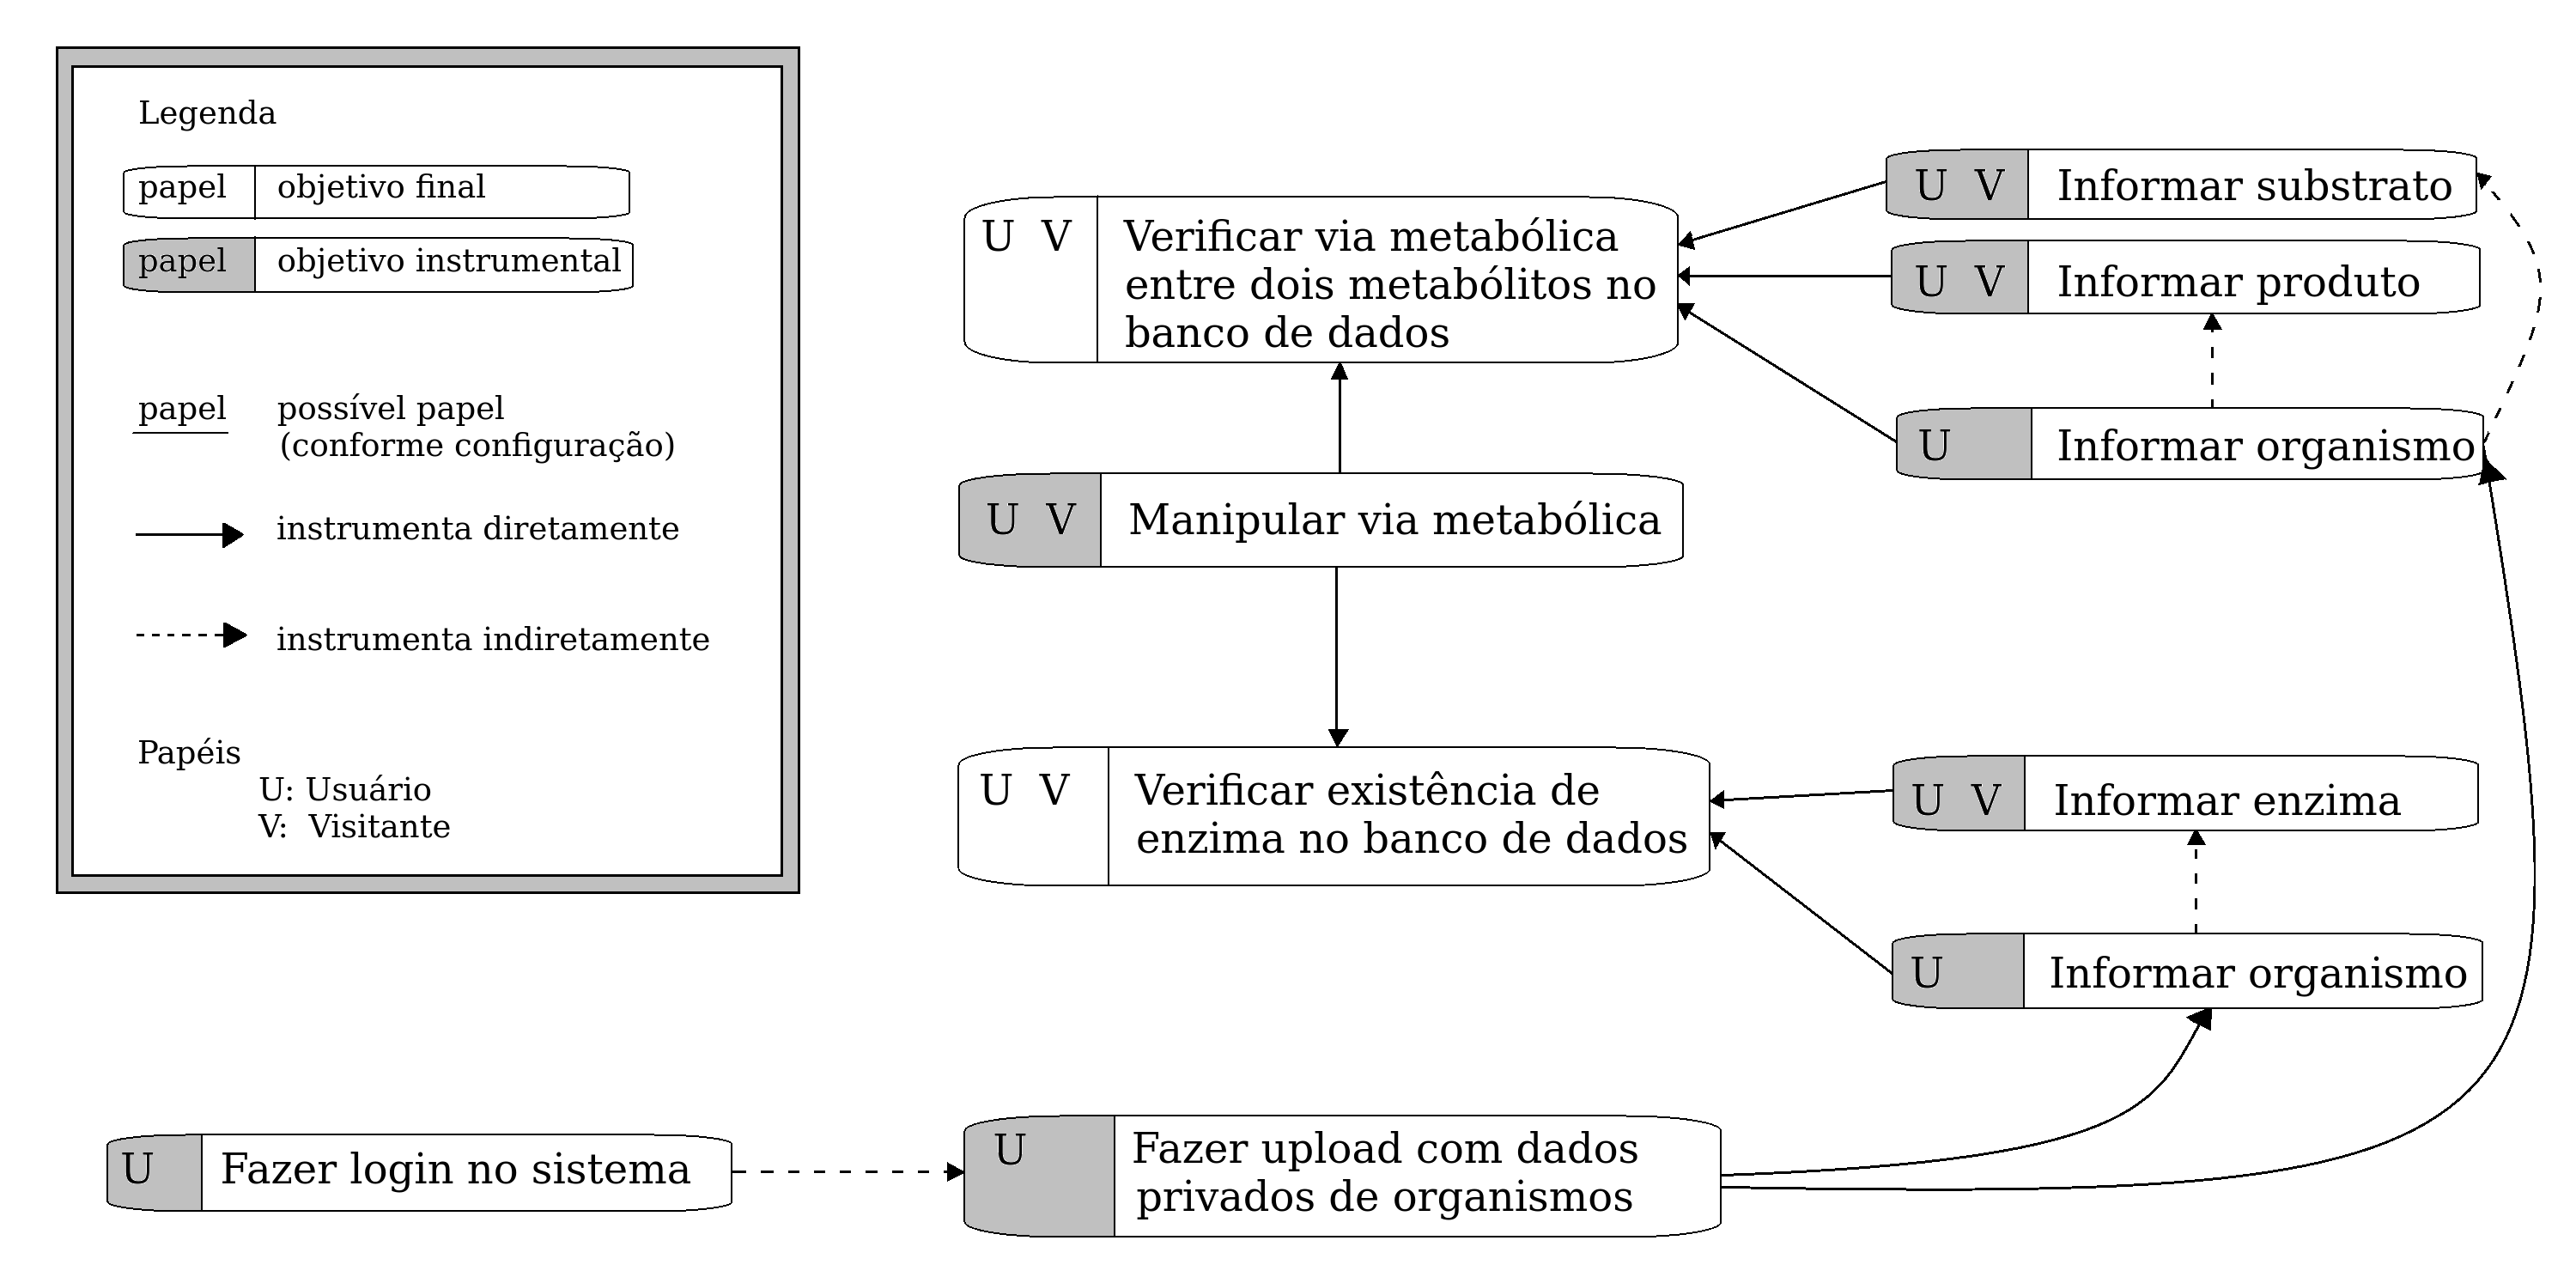
\includegraphics[width=1\textwidth]{mapaDeObjetivos.png}
	\caption{Mapa de objetivos finais e intrumentais.}
	\label{fig:mapaDeObjetivos}
\end{figure} 

\subsection{Modelagem de Tarefas}

\indent A partir do mapa de objetivos, têm-se uma ideia geral da navegação do \textit{site}, uma vez que foi feito um mapeamento generalizado das sequências de passos para atingi-los. O propósito da modelagem de tarefas é, portanto, estabelecer essa sequências de passos de maneira específica para cada objetivo final. 

\indent No caso, foram elaborados dois objetivos finais: Verificar via metabólica entre dois metabólitos no banco de dados; verificar existência de enzima no banco de dados. Entretanto a pequisa pode ser feita tanto no banco de dados completo do 2Path, quanto na rede metabólica construída para um organismo específico. Assim, esses objetivos finais foram subdivididos em dois na modelagem de tarefas: Verificar se uma enzima está no banco de dados público do 2Path (Figura \ref{fig:objetivo_enzyma}); verificar se uma enzima está no banco de dados privado (Figura \ref{fig:objetivo_enzyma_organismo}); verificar se há uma via entre dois metabólitos no banco de dados público (Figura \ref{fig:objetivo_pathway}); verificar se há uma via metabólica no banco de dados privado (Figura \ref{fig:objetivo_pathway_organismo});

\begin{figure}[!h]
    \centering
    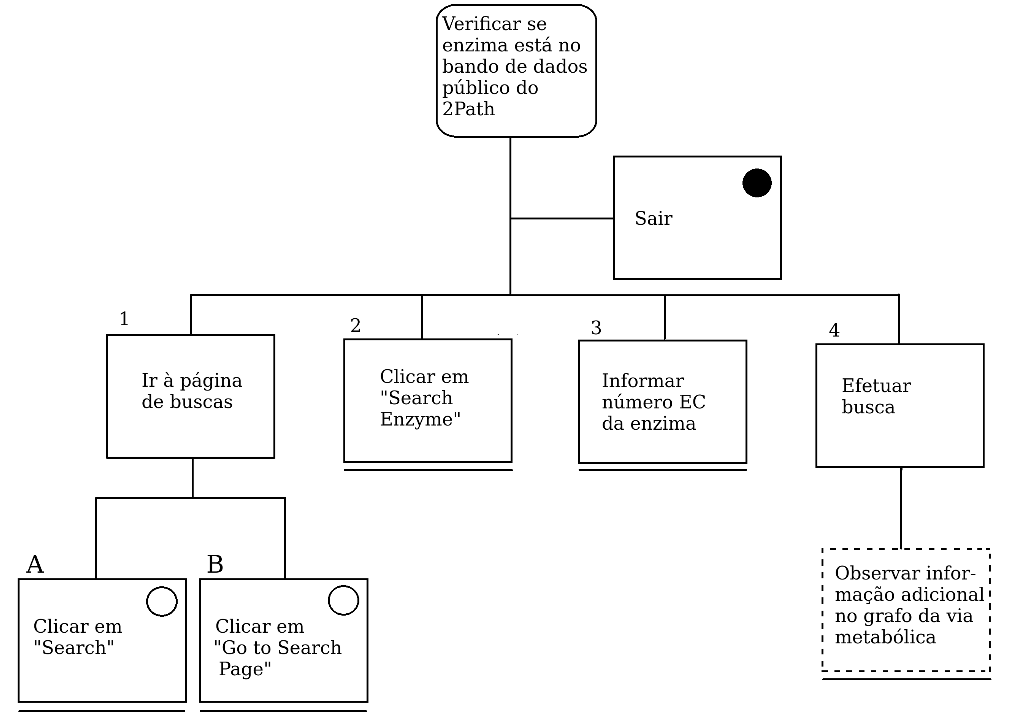
\includegraphics[width=0.8\textwidth]{objetivo_enzima.png}
    \caption{Objetivo de pesquisar enzima no banco de dados completo do 2Path.}
    \label{fig:objetivo_enzyma}
\end{figure}

\newpage
\begin{figure}[!h]
    \centering
    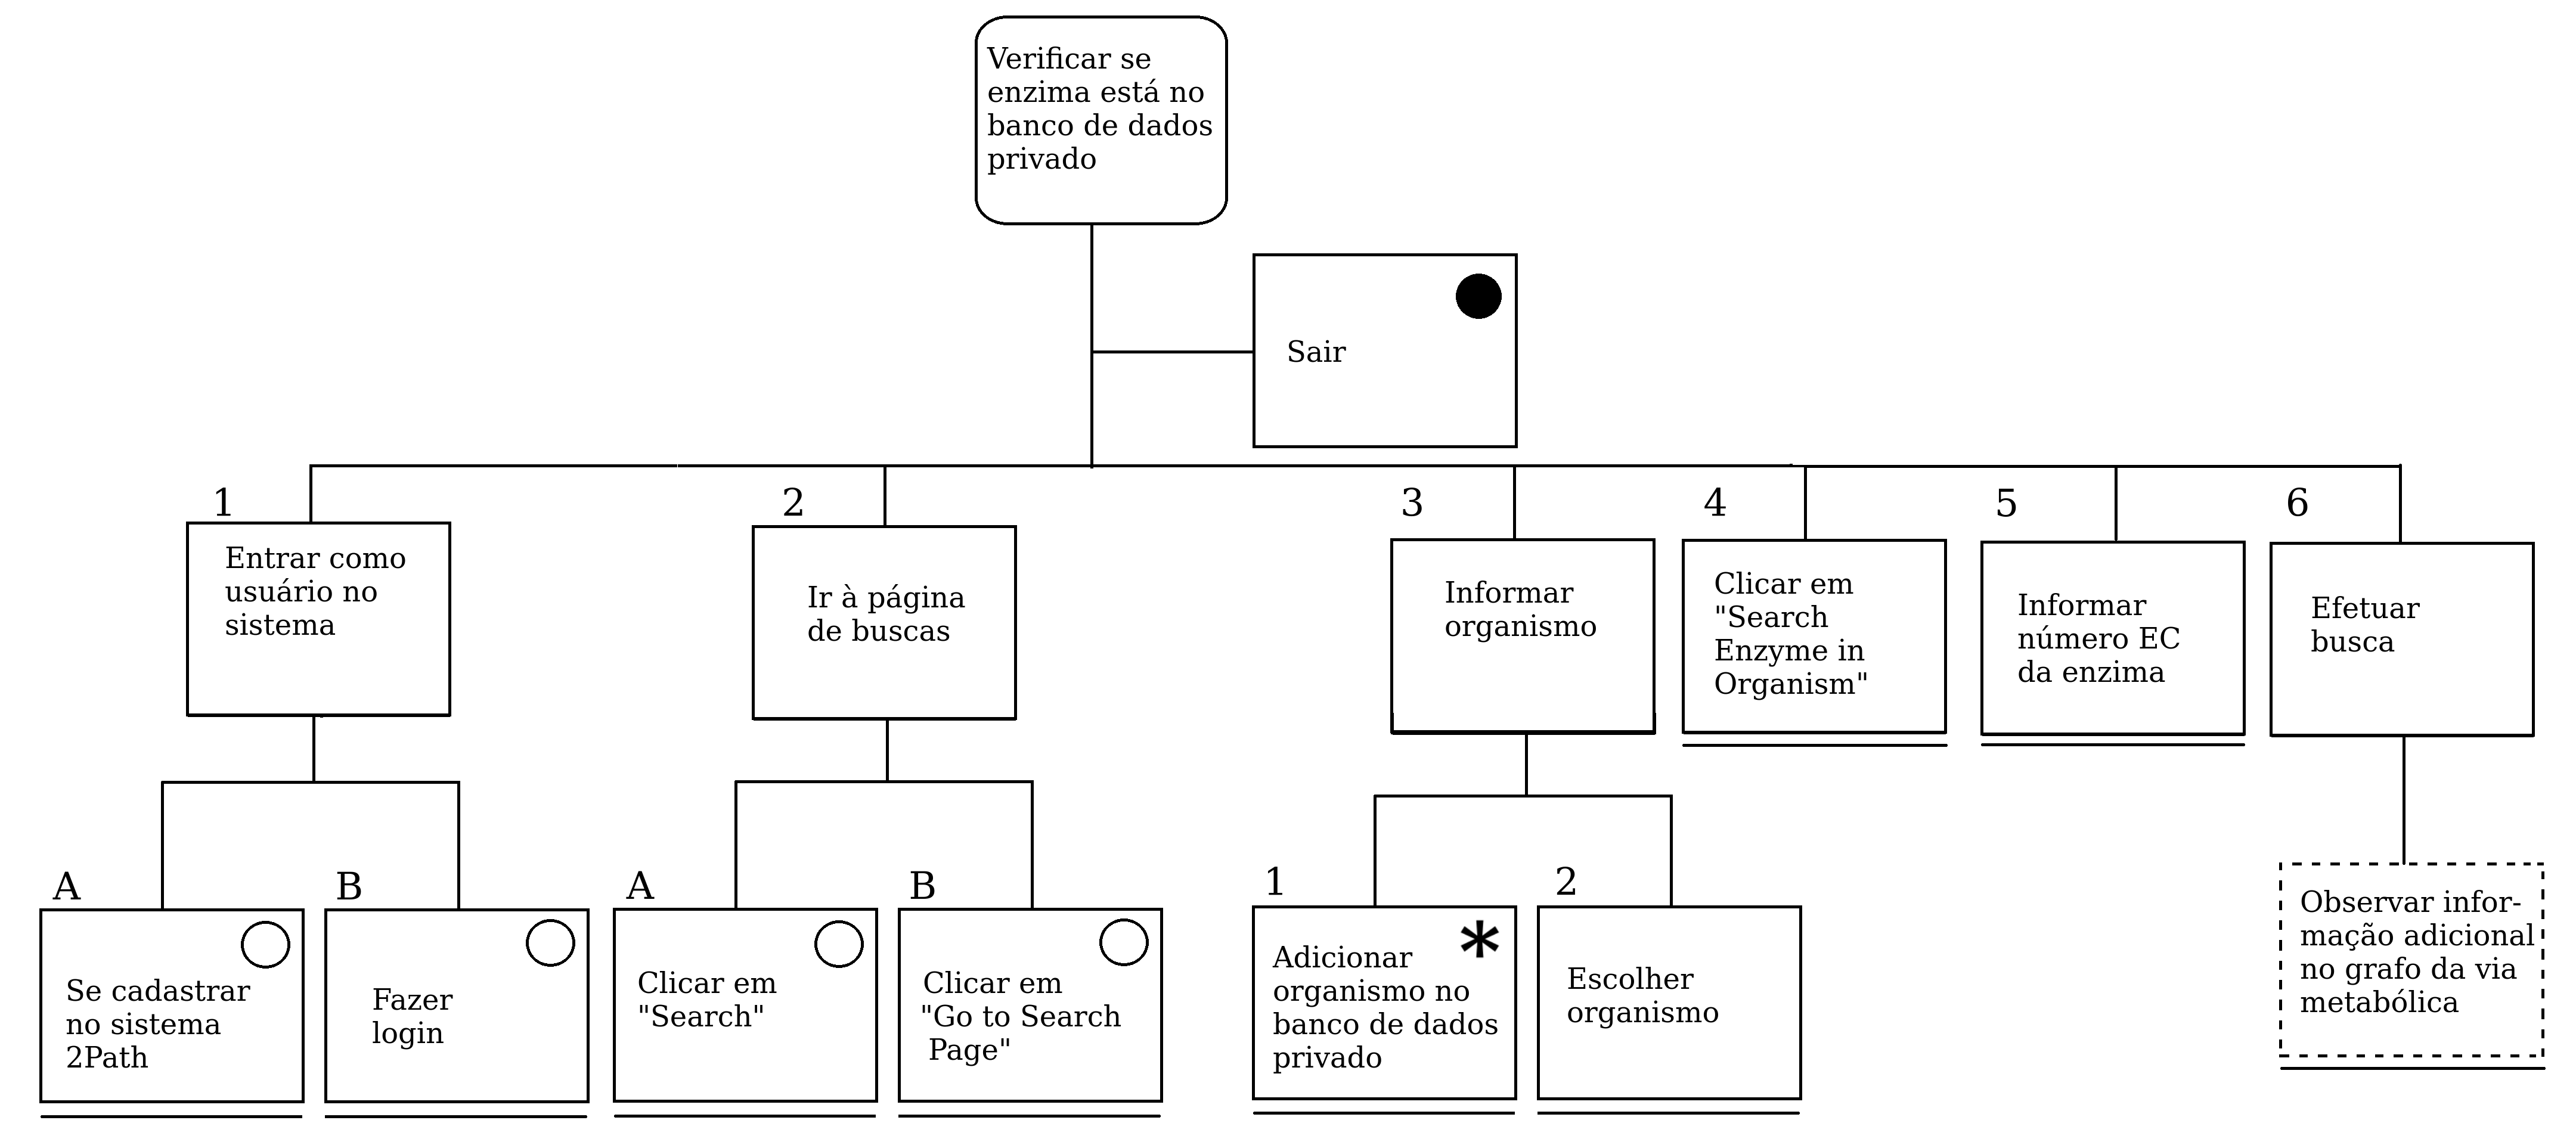
\includegraphics[width=1\textwidth]{objetivo_enzima_organismo.png}
    \caption{Objetivo de pesquisar enzima no banco de dados específico para a rede metabólica construída a partir do organismo do usuário.}
    \label{fig:objetivo_enzyma_organismo}
\end{figure}

\begin{figure}[!h]
    \centering
    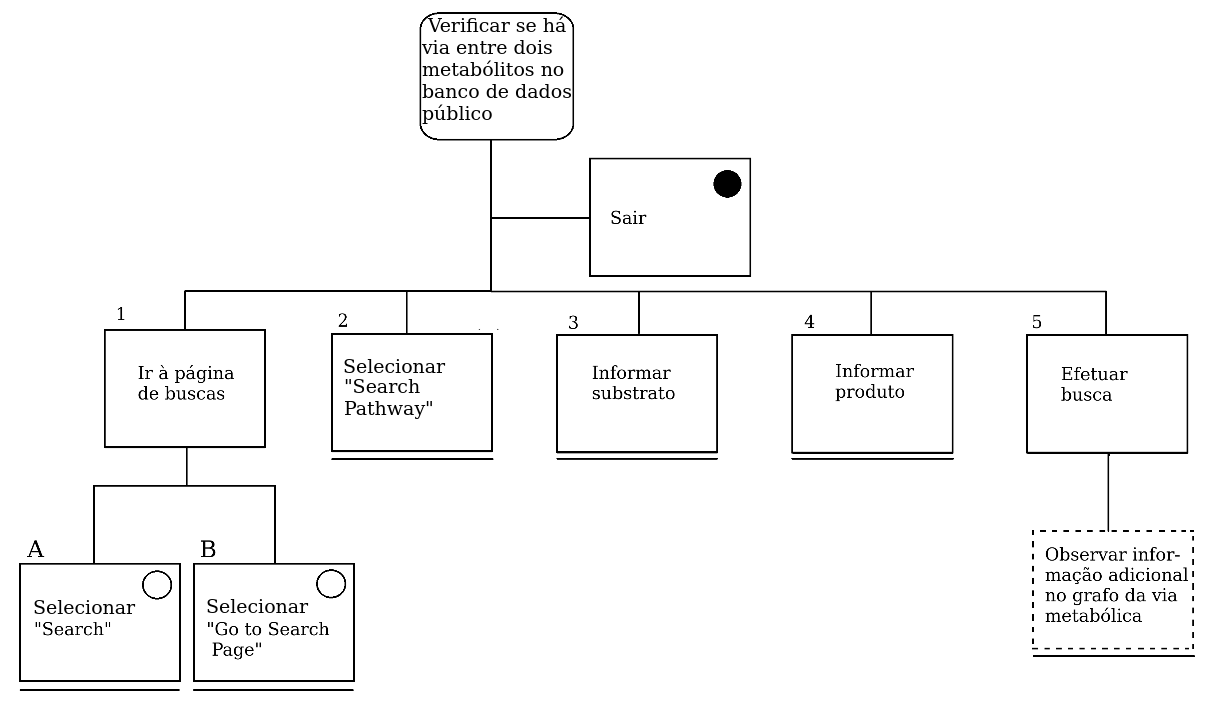
\includegraphics[width=1\textwidth]{objetivo_pathway.png}
    \caption{Objetivo de pesquisar via metabólica entre substrato e produto no banco de dados completo do 2Path.}
    \label{fig:objetivo_pathway}
\end{figure}
\break
\begin{figure}[!h]
    \centering
    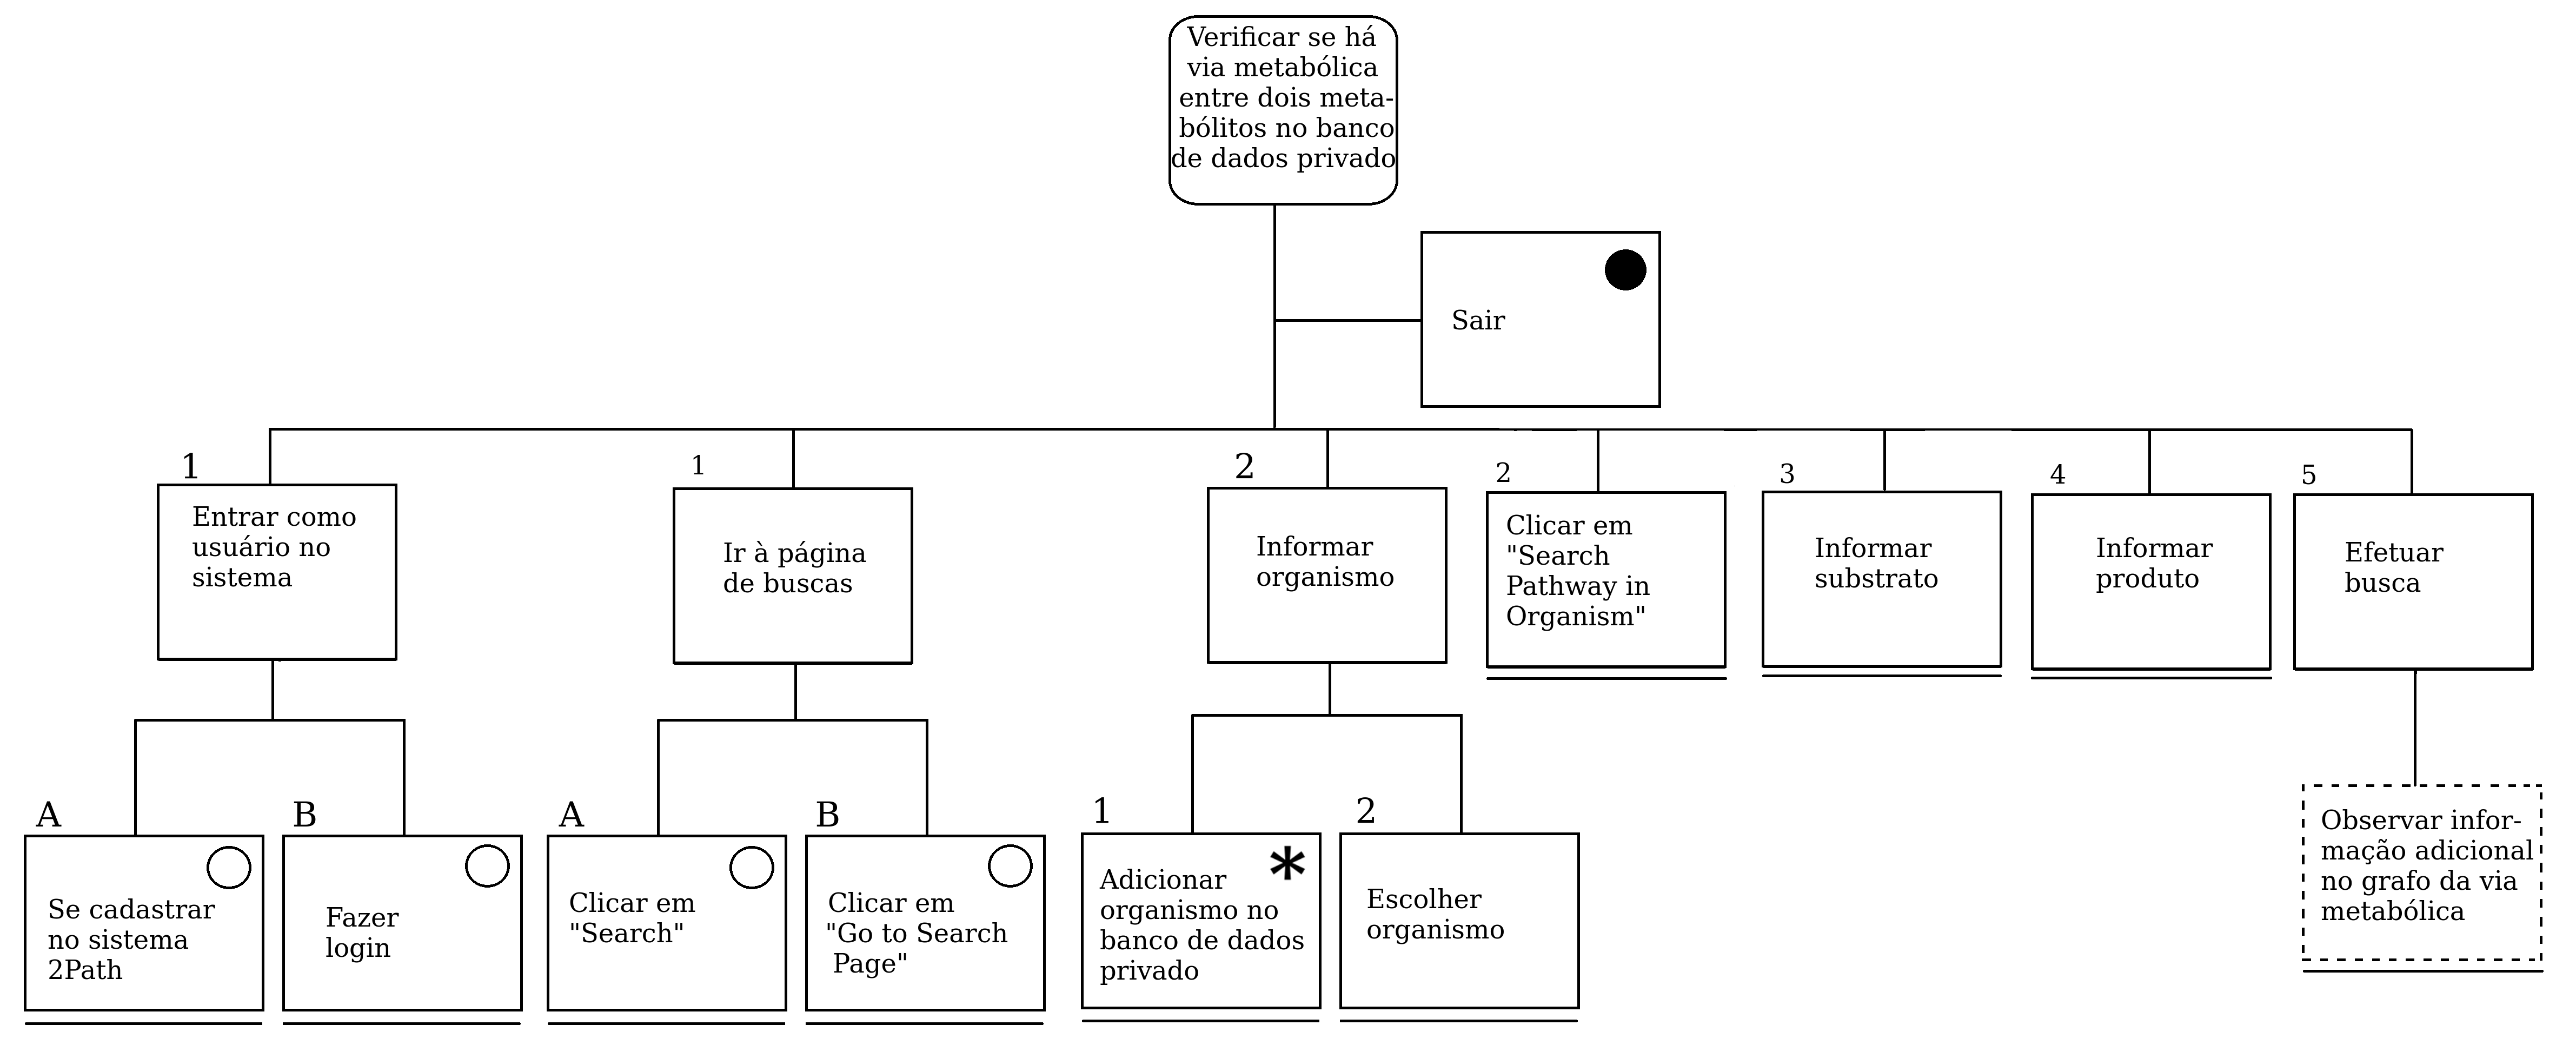
\includegraphics[width=1\textwidth]{objetivo_pathway_organismo.png}
    \caption{Objetivo de pesquisar via metabólica entre substrato e produto no banco de dados  específico para a rede metabólica construída a partir do organismo do usuário.}
    \label{fig:objetivo_pathway_organismo}
\end{figure}

\subsection{Tratamento de Rupturas na Comunicação}

\indent A Tabela \ref{prevencaoRecuperacao:2Path} apresenta as medidas tomadas para prevenção e recuperação de falhas de comunicação na interface do 2Path, assim como especificado no Capítulo 2. Nela, PP significa a prevenção passiva, PA siginifica prevenção ativa e RA significa recuperação apoiada. 

\indent Não houve nenhum tipo de prevenção apoiada, pois não foi observado nenhum tipo de interação que o usuário possa fazer que cause dano grave, por exemplo, excluir um arquivo. À medida que este projeto seja desenvolvido, esse tipo de prevenção pode ser aplicada, por exemplo, ao se tratar o \textit{upload} de um arquivo FASTA, onde o projetista deverá verificar se existe um organismo com o mesmo nome já no banco de dados privado do usuário. 

\indent Também não foi constatada a necessidade de implementar captura de erro, uma vez que todas as possíveis rupturas observadas são tratáveis por meio de mensagens de erro.

\indent 
\begin{table}
\centering
\caption{Campos de entrada e manipulação dos usuários do sistema 2Path. Observe que não houve prevenção nem recuperação da manipulação de vias metabólicas, pois o usuário não entra com dados nem altera dados, apenas visualiza e interage com o grafo utilizando o \textit{mouse}.} \label{prevencaoRecuperacao:2Path}
\begin{tabular}{|l|c|c|}
\hline
{\cellcolor[HTML]{DFDFDF}\textbf{Signo}} &  {\cellcolor[HTML]{DFDFDF}\textbf{Prevenção}} &  {\cellcolor[HTML]{DFDFDF}\textbf{Recuperação}}\\ \hline
\specialcell{Seleção de\\organismo}  & \specialcell{\textbf{PA}: Campo obrigatório com\\indicador ``*'' para\\ formulários ``\textit{Search Enzyme}\\\textit{in Organism}'' e  ``\textit{Search}\\\textit{Pathway in Organism}''. Caso\\o usuário esqueça de selecionar\\este campo, o organismo\\escolhido será o primeiro em\\ordem alfabética.} & -  \\ \hline

\specialcell{Seleção de\\enzima} & \specialcell{\textbf{PP}: Campo obrigatório com\\indicador ``*'';\\\textbf{PP}: Campo possui função\\\textit{auto-complete}, que fornece\\ao usuário todos os\\números EC existentes} & \specialcell{\textbf{RA}: Mensagem de texto em vermelho \\aparece acima do formulário informando\\o usuário de que o campo obrigatório\\não foi preenchido: ``\textit{Enzyme: Validation}\\\textit{ Error: Value is required}''.} \\ \hline

\specialcell{Seleção de\\substrato} & \specialcell{\textbf{PP}: Campo obrigatório com\\indicador ``*'';\\\textbf{PP}: Campo possui função\\\textit{auto-complete}, que fornece\\ao usuário todos os\\compostos existentes no\\2Path} & \specialcell{\textbf{RA}: Mensagem de texto em vermelho \\aparece acima do formulário informando\\o usuário de que o campo obrigatório\\não foi preenchido: ``\textit{From: Validation}\\\textit{Error: Value is required.}''.\\O ``From'' significa que a via\\tem início neste metabólito} \\ \hline

\specialcell{Seleção de\\produto} & \specialcell{\textbf{PP}: Campo obrigatório com\\indicador ``*'';\\\textbf{PP}: Campo possui função\\\textit{auto-complete}, que fornece\\ao usuário todos os\\compostos existentes no\\2Path} & \specialcell{\textbf{RA}: Mensagem de texto em vermelho \\aparece acima do formulário informando\\o usuário de que o campo obrigatório\\não foi preenchido: ``\textit{To: Validation}\\\textit{Error: Value is required.}''.\\O ``To'' significa que a via\\finaliza neste metabólito} \\ \hline

\specialcell{Manipulação\\da via\\metabólica} & - & - \\ \hline
\end{tabular}
\end{table}

% =========================================================================================

\section{Implementação da Interface} \label{implementacao}


\indent O sistema desenvolvido para este projeto é uma aplicação web chamada \textit{EnzymeGraph}. Nesta seção serão apresentadas as linguagens e ferramentas utilizadas no desenvolvimento do \textit{website}, as características, funcionalidades e limites do sistema e, por fim, as dificuldades enfrentadas na implementação do projeto.

\subsection{Detalhes de Implementação}

\indent O sistema foi desenvolvido no amibiente de desenvolvimento integrado \textit{open source} Eclipse Java EE - \textit{Java Platform, Enterprise Edition}, versão Mars 4.5.2. Para simplificar a obtenção das dependências do projeto, ou seja, pacotes de arquivos java (extensão .jar), foi utilizada o Apache Maven\footnote{\textit{Software} de gerenciamento de projeto e ferramenta de compreensão de programa.}. Este \textit{software} opera sobre o arquivo \textit{pom.xml} (\textit{Project Object Model}) e contém as especificações de cada projeto que se tornará dependência do sistema em desenvolvimento, além de outros aspectos do código. O servidor selecionado para hospedagem local, \textit{localhost} porta 8080, do sistema foi o Apache TomCat versão 7.0.

\indent As páginas da aplicação foram desenvolvidas na linguagem de marcação XHTML, \textit{Extensible Hypertext Markup Language}, e a estilização em CSS, \textit{Cascading Style Sheets}. Para conexão entre \textit{front-end} e \textit{back-end} foram utilizados JSF\footnote{Especificação Java para criação de componentes de interface de aplicação \textit{web}.}, Primefaces\footnote{Biblioteca com uma coleção de componentes de interface voltadas para JSF.}, e Javascript, para a construção do grafo de vias metabólicas.

\indent Em javascript, foi utilizada a bilioteca D3 na apresentação das vias metabólicas na tela. Essa biblioteca permite que a construção de um grafo a partir de um arquivo ou \textit{string} no formato JSON com os vetores \textit{nodes} para os nós e \textit{links} para as arestas. Não houve padrão definido para a escolha das cores de cada nó, apresentadas na Figura~\ref{fig:nodeslinksD3}.

\begin{figure}[!h]
    \centering
    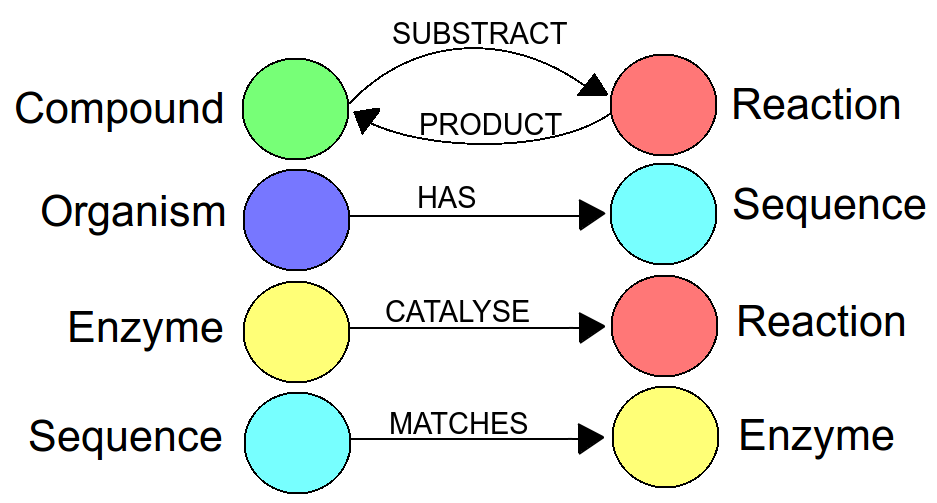
\includegraphics[width=0.6\textwidth]{nodeslinksD3.png}
    \caption{Diagrama geral de uma via metabólica na interface do 2Path.}
    \label{fig:nodeslinksD3}
\end{figure}

\indent O banco de dados em grafo Neo4j~\cite{waldeyr} foi utilizado no sistema, pois o próprio 2Path foi desenvolvido no mesmo. Devido à facilidade de implementação do mesmo em Java e da alta usabilidade de sua interface, foi relativamente simples implementar as \textit{queries} de busca e fazer a conexão em Java. As \textit{queries} foram escritas em \textit{CYPHER}, linguagem nativa do Neo4j. Como o banco não é relacional, essa linguagem não tem a estrutura do SQL, porém foi elaborada para facilitar buscas que realizam travessia em grafos. 

\indent O Neo4j, porém, retorna em suas transações uma \textit{string} em formato JSON que não é compatível com o especificado pelo D3 (Data-Driven Documents). Nesse caso, foi feito um tradutor para a construção de uma nova \textit{string} compatível. Os dados passados de uma página para a outra, inclusive essa string em JSON, são todos armazenados em uma sessão, cujo ciclo de vida é determinado pelo JSF.

\subsection{Interface do Sistema}

\indent A implementação do \textit{front-end} resultou nas figuras a seguir. Todos os elementos estão em inglês, pois o sistema criado pode ser utilizado mundialmente. A Figura \ref{fig:2path_home} mostra a página inicial, que possui uma breve explicação sobre terpenoides, sobre o sistema 2Path e sobre as possíveis buscas que o usuário pode realizar. O menu ao topo está em todas as páginas do sistema. Nele é possível navegar até a página inicial (Home), página sobre terpenoides (Terpenoids), página de busca (Search), página sobre o 2Path (About) e, por fim, página de ajuda (Help).

\begin{figure}[!h]
    \centering
    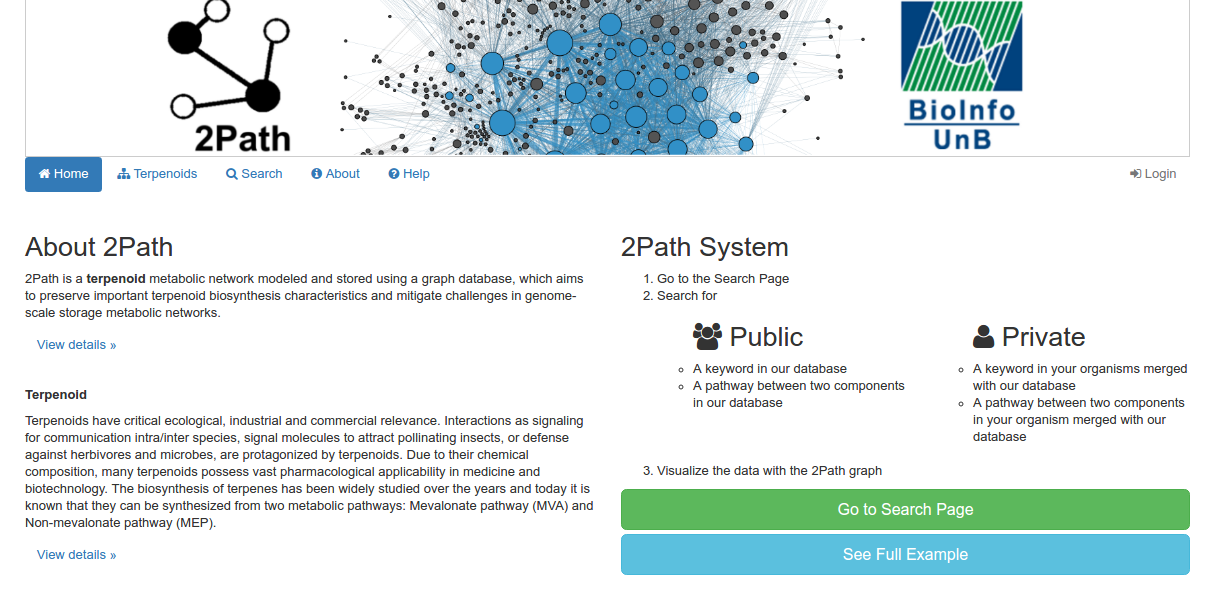
\includegraphics[width=1\textwidth]{2path_home.png}
    \caption{Página inicial do 2Path.}
    \label{fig:2path_home}
\end{figure}

\indent A Figura \ref{fig:2path_search} apresenta a página de busca principal, onde a partir dela é possível fazer as quatro tipos de buscas: por enzima no 2Path; por enzima no organismo; por via metabólica no 2Path e por via metabólica no organismo.

\begin{figure}[!h]
    \centering
    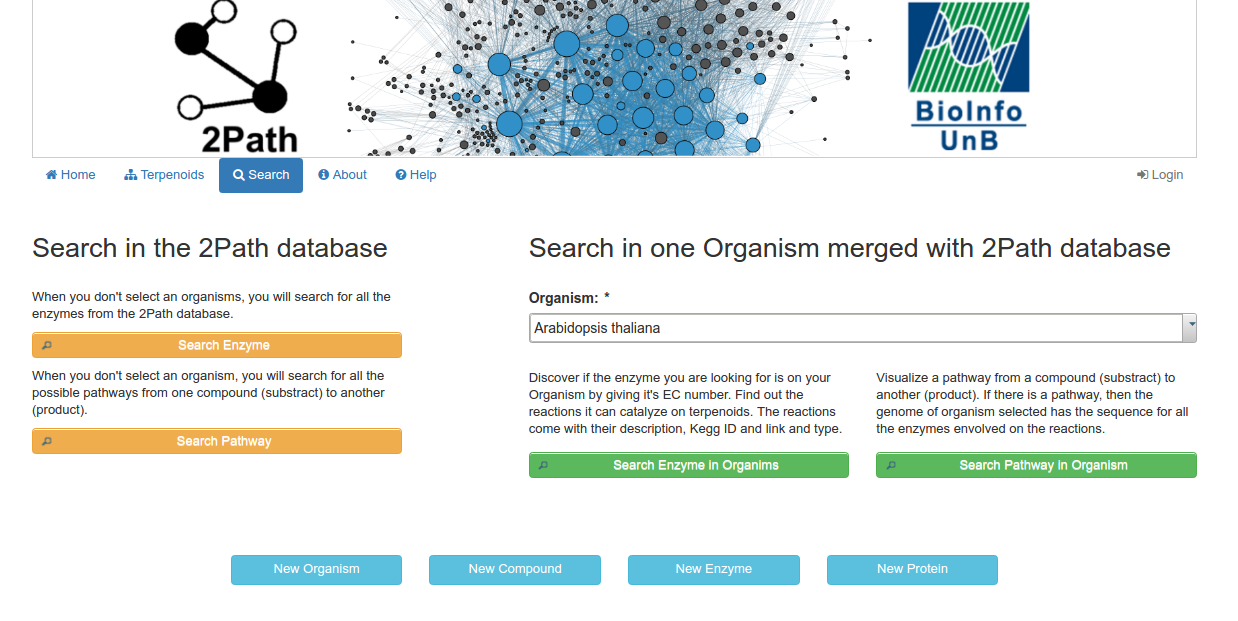
\includegraphics[width=1\textwidth]{2path_search.png}
    \caption{Página principal de busca no 2Path.}
    \label{fig:2path_search}
\end{figure}

\indent Em relação às buscas específicas, decidiu-se apresentar o grafo das vias metabólicas em uma página separada da busca, pois ele poderia ficar extenso e complexo. Nesse sentido, a busca de fato é realizada em uma página intermediária, que apenas responde se a enzima/via foi encontrada ou não. Caso o usuário queira saber detalhes sobre a mesma, ele deve selecionar o botão \textit{View Interactive Data}. A Figura \ref{fig:2path_enzyme} apresenta um exemplo de busca pela enzima \textit{2.7.7.60} no banco de dados completo do 2Path.

\begin{figure}[!h]
    \centering
    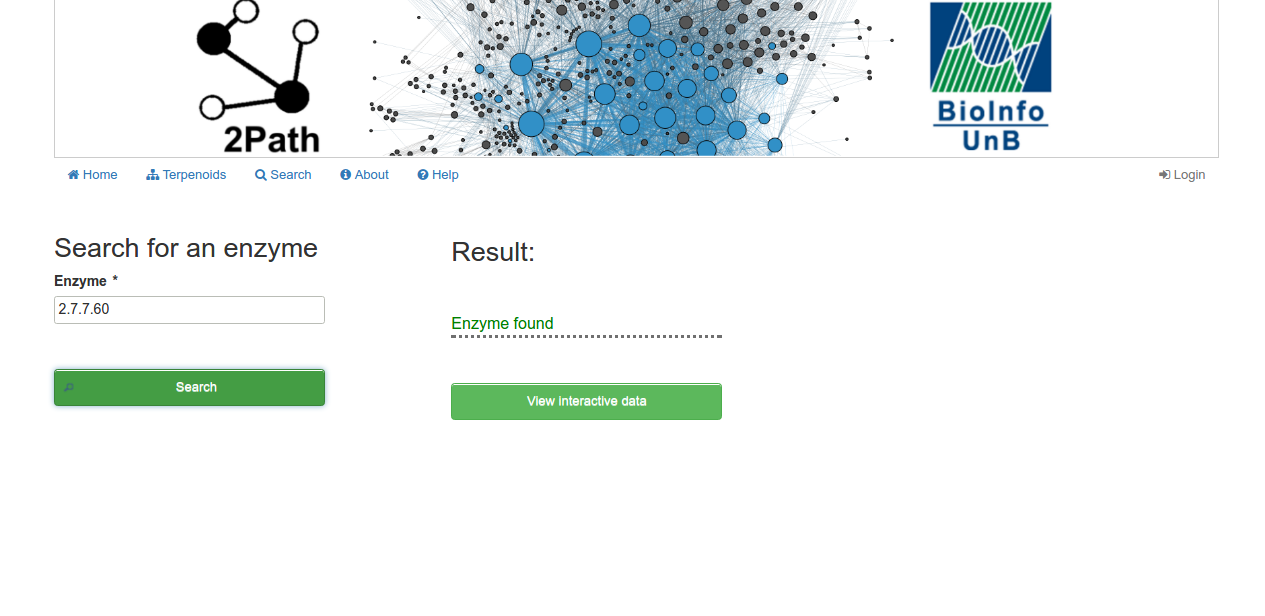
\includegraphics[width=1\textwidth]{2path_enzyme.png}
    \caption{Página de busca por enzima no banco completo}
    \label{fig:2path_enzyme}
\end{figure}

\indent Uma vez que essa enzima foi encontrada, o grafo da Figura \ref{fig:2path_enzyme_graph} apresenta o substrato (\textit{2-C-Methyl-D-erythritol 4-phosphate}) que ela recebe e o produto (\textit{4-(Cytidine 5'-diphospho)-2-C-methyl-D-erythritol}) que ela produz. 

\begin{figure}[!h]
    \centering
    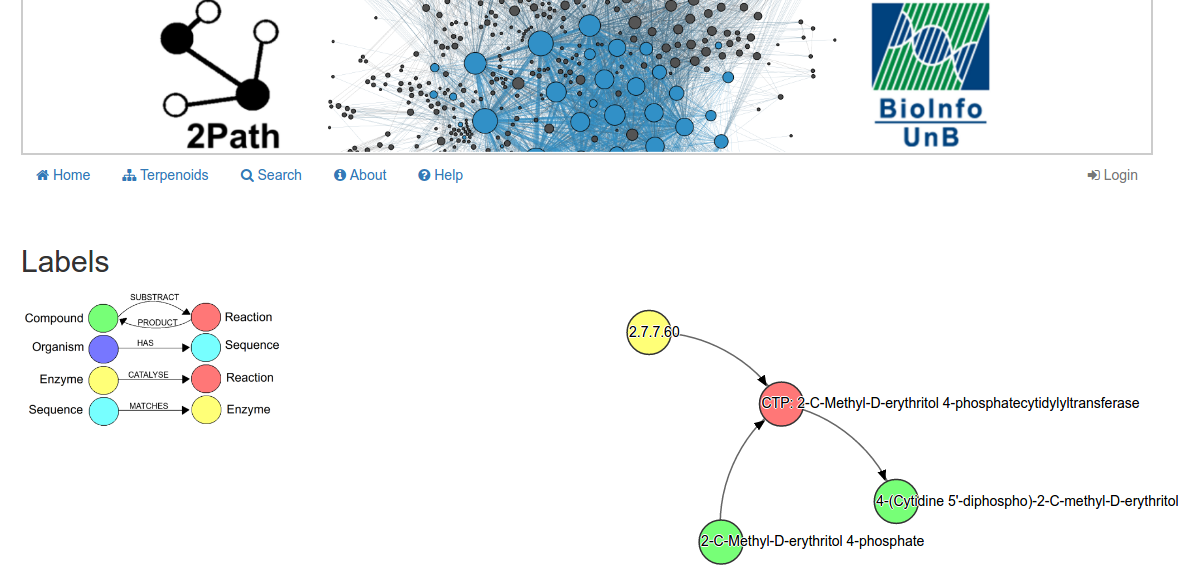
\includegraphics[width=1\textwidth]{2path_enzyme_graph.png}
    \caption{Página de apresentação da reação bioquímica catalisada pela enzima buscada.}
    \label{fig:2path_enzyme_graph}
\end{figure}

\indent A Figura \ref{fig:2path_pathway_org} apresenta um exemplo de busca por via metabólica entre os compostos \textit{1-Deoxy-D-xylolose 5-phosphate} e \textit{2-phospho-4-(cytidine 5'-diphospho)-2-C-methyl-D-erythritol} no organismo \textit{Arabidopsis thaliana}.

\begin{figure}[!h]
    \centering
    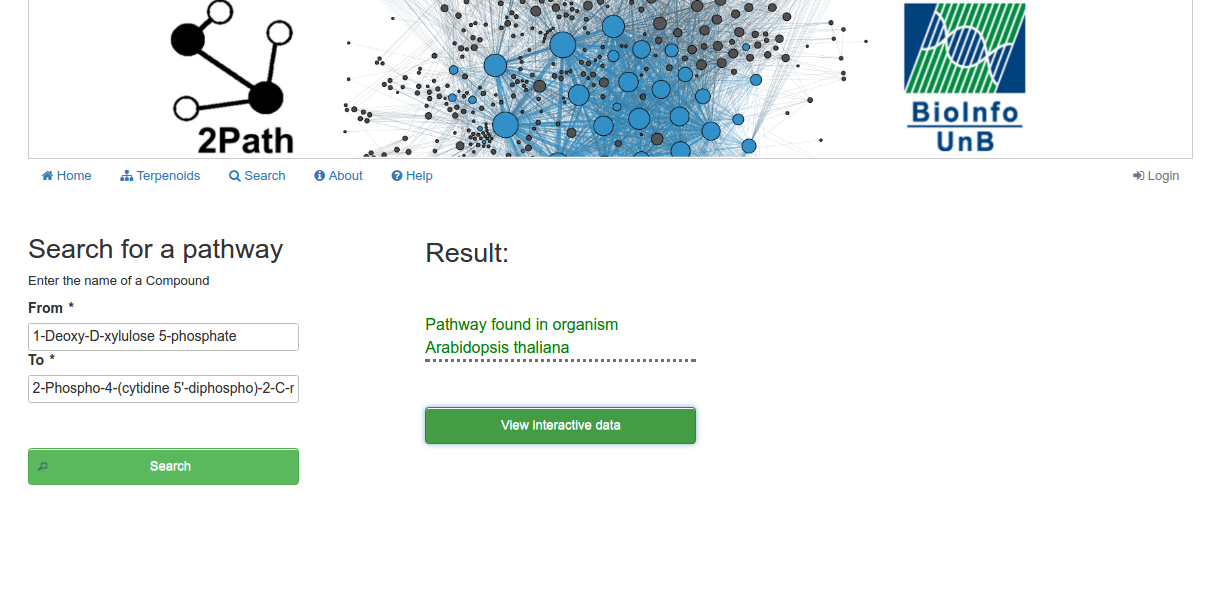
\includegraphics[width=1\textwidth]{2path_pathway_org.png}
    \caption{Página de busca por via metabólica no banco de dados formado para o organismo \textit{Arabidopsis thaliana}.}
    \label{fig:2path_pathway_org}
\end{figure}

\indent O grafo gerado para esta via é representado na Figura \ref{fig:2path_pathway_graph}.

\begin{figure}[!h]
    \centering
    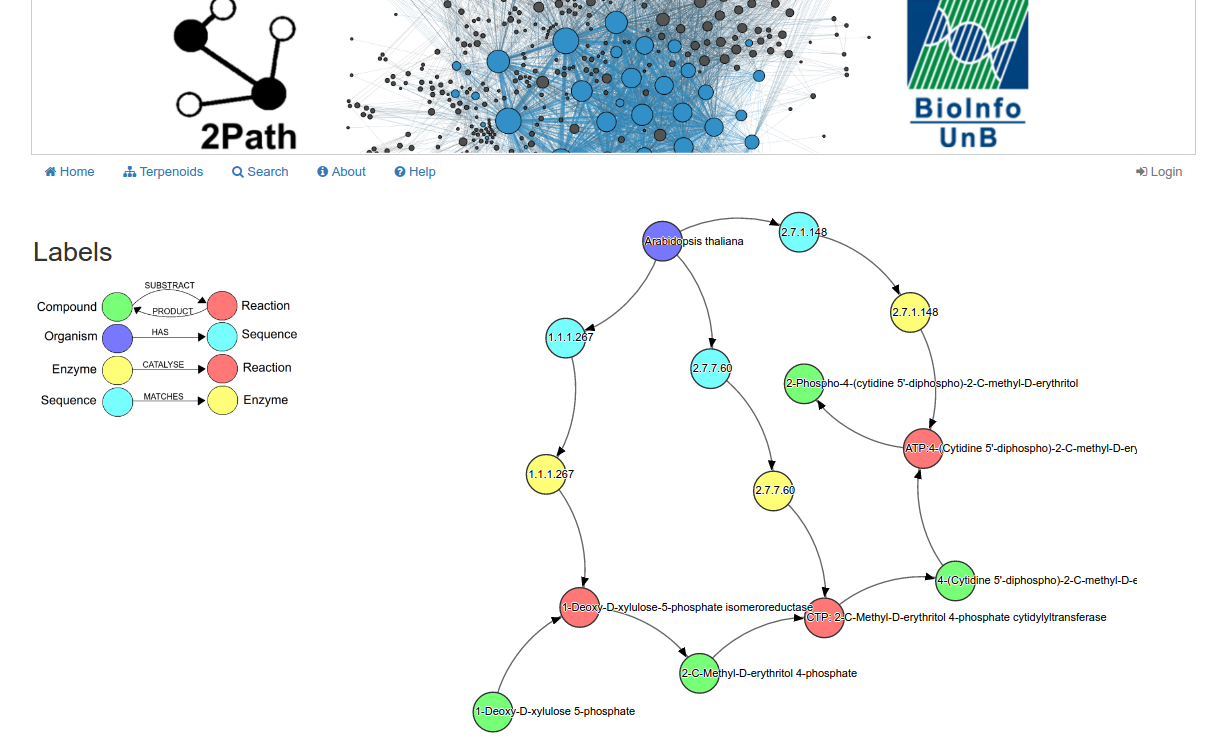
\includegraphics[width=1\textwidth]{2path_pathway_graph.png}
    \caption{Página de apresentação da via metabólica de reações que ocorrem no organismo \textit{Arabidopsis thaliana}.}
    \label{fig:2path_pathway_graph}
\end{figure}

\section{Projeto de Avaliação} \label{avaliacao}

\indent Os testes foram realizados no Laboratório de Bioinformática do Departamento de Biologia Celular, Instituto de Ciências Biológicas da Universidade de Brasília. Três biólogos foram selecionados para participar do teste descritos pelo Método de Avaliação de Comunicabilidade no capítulo 2. A identidade dos mesmos será preservada por questão de privacidade.

\indent Primeiramente, cada biólogo respondeu ao questionário do Apêndice \ref{questionario_dados_pessoais}. Ele é necessário para analisar se o perfil do usuário tem alguma relação com a facilidade com que o mesmo possui ao realizar um tarefa proposta no sistema. Para isso, é importante conhecer a formação acadêmica do usuário, bem como sua atuação profissional. Além disso, foram solicitadas informações sobre a frequência em que ele utiliza ferramentas interativas e o nível de conhecimento a respeito de redes metabólicas. 

\indent Após responderem o questionário, cada usuário fez o teste separadamente, sem acesso às respostas de outro usuário para que o teste não perca a legitimidade. Apenas um avaliador guiou os usuários e apenas um computador foi utilizado para os testes. Assim, os testes foram realizados em sequência. Foi utilizado o computador pessoal do avaliador para a realização das tarefas, ao invés de um computador do Laboratório de Bioinformática, uma vez que o ambiente de teste já está configurado corretamente no computador pessoal. Configurar o ambiente em um outro computador poderia levar em torno de 2 horas, levando em consideração que seria necessário fazer \textit{download} da IDE Eclipse e do banco de dados Neo4j.

\indent Durante a realização das tarefas, foram filmadas a tela do computador, o \textit{mouse} / \textit{mousepad}, o teclado e as mãos dos usuários. Foram apresentadas aos usuários, um de cada vez, as 13 etiquetas descritas no capítulo 2 para que eles entendam o propósito do teste. Não houve comunicação entre avaliador e usuário durante a realização das tarefas.

\indent Foram realizadas 5 tarefas, descritas no Apêndice \ref{tarefas}. As primeiras três envolvem buscar por enzimas em um organismo. Considerou-se que o organismo já havia sido processado pelo sistema do \textit{2Path} e as sequências de seu arquivo FASTA já haviam sido ligadas às enzimas correspondentes do banco de dados. Assim, o usuário deveria apenas selecionar o organismo listado na página de busca e pesquisar pelas enzimas. As outras duas tarefas envolvem buscar por vias metabólicas no banco de dados inteiro do \textit{2Path}.

\indent Após a tarefa, os usuários responderam ao questionário do Apêndice \ref{questionario_interface}, que visa coletar a opinião dos mesmos a respeito do projeto de interface. Estes dados, juntamente com as etiquetas listadas para cada usuário, fornecem uma base de informação para análise e a re-implementação aperfeiçoada do sistema.

\indent Por fim, foi apresentada a nova proposta de interface do banco de dados 2Path, de acordo com as necessidades dos usuários e contemplando novos recursos que devem aumentar os quatro critérios de qualidade: usabilidade, experiência de usuário, acessibilidade e comunicabilidade.